\documentclass[11pt,a4paper]{article}
\usepackage{graphicx}
\usepackage{subfigure}
\usepackage{amsmath}
\usepackage{makecell}
\usepackage[utf8]{inputenc}
\usepackage{listings} %放代码
\usepackage{xcolor} %代码着色宏包
\usepackage{color}
\usepackage{xeCJK}
\usepackage{float}

%好像是数学的包
\usepackage{amsmath}
\usepackage{amssymb}
\usepackage{mathrsfs}
%页面布局包
\usepackage{geometry}
%画图包
\usepackage{tikz}
%画图背景包
\usetikzlibrary{backgrounds}

\geometry{left=3.0cm, right=3.0cm, top=3cm, bottom=3cm}

%自定义命令
\newcommand{\psiG}{\psi_{G}}
%在tikz中画一个顶点
%#1:node名称
%#2:位置
%#3:标签
\newcommand{\newVertex}[3]{\node[circle, draw=black, line width=1pt, scale=0.8] (#1) at #2{#3}}
%在tikz中画一条边
\newcommand{\newEdge}[2]{\draw [black,very thick](#1)--(#2)}
%在tikz中放一个标签
%#1:名称
%#2:位置
%#3:标签内容
\newcommand{\newLabel}[3]{\node[line width=1pt] (#1) at #2{#3}}


\title{Introduction to Computing Systems\\Homework 1}
\author{PB18111697 王章瀚}

\begin{document}
	\maketitle
	\section{(Adaptedfromproblem1.5inthetextbook)}
	The answers are as following.
	\subsection*{a.}
	\begin{figure}[H]
		\centering
		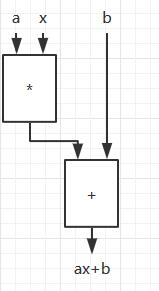
\includegraphics[scale=0.7]{1_a.jpg}
		\caption{1.a\ $ax+b$}
		\label{1.a}
	\end{figure}\par
	\subsection*{b.}
	\begin{figure}[H]
		\centering
		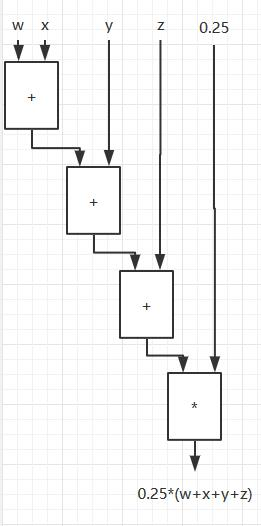
\includegraphics[scale=0.7]{1_b.jpg}
		\caption{1.b\ average of $x, y, z, w$}
		\label{1.b}
	\end{figure}\par
	\subsection*{c.}
	\begin{figure}[H]
		\centering
		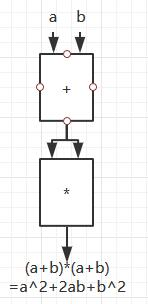
\includegraphics[scale=0.7]{1_c.jpg}
		\caption{1.c\ $a^{2}+2ab+b^{2}$}
		\label{1.c}
	\end{figure}\par
	\subsection*{d.}
	\begin{figure}[H]
		\centering
		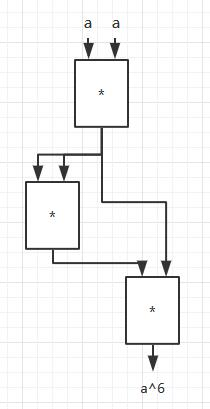
\includegraphics[scale=0.7]{1_d.jpg}
		\caption{1.d\ $a^{6}$}
		\label{1.d}
	\end{figure}\par
	\subsection*{e.}
	\begin{figure}[H]
		\centering
		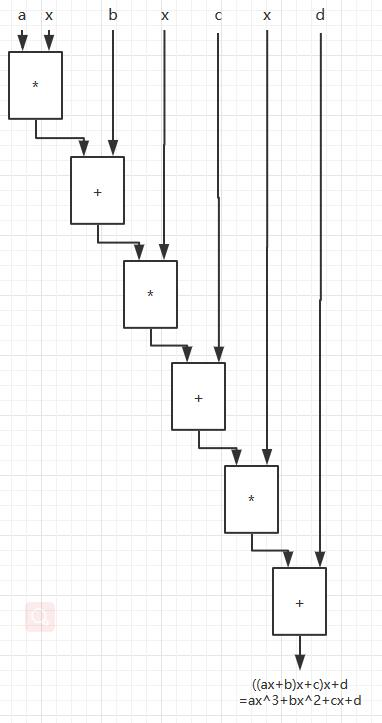
\includegraphics[scale=0.7]{1_e.jpg}
		\caption{1.e $ax^{3}+bx^{2}+cx+d$}
		\label{1.e}
	\end{figure}\par


	\section{(Adaptedfromproblem1.12inthetextbook)}
	\subsection*{a.}
	\underline{No. It lacks definiteness.} This description ignored the sequence of all steps, which means we can add row1 to row2 then row1 to row4, as well as the other sequence. Even though all kinds of sequences can result the same answer, it still lacks definiteness.
	\subsection*{b.}
	\underline{No. It lacks finiteness.} It is obviouly that there are an infinite number of prime numbers and natural numbers, which means the algorithm can't be finite.
	\subsection*{c.}
	\underline{Yes. It doesn't lack any of definiteness, effective computability or finiteness.}
	\subsection*{d.\textcolor{red}{no. finiteness}}
	\underline{No. It seems to lack the definiteness and the effective computability.} First, on each flip, the state of the coin is unpredictable, which renders the description missing definiteness. What's more, the computers nowadays cannot really generate a random number, making the item uncomputable.
	\subsection*{e.\textcolor{red}{no. x-1. finiteness}}
	\underline{The item is an algorithm when and only when the number given is a positive integer.} Suppose the number firstly given as x. After the first 6 steps, the number becomes x-1. This ensures all positive integer can finally become 0, while other numbers can't; so if the number given isn't a positive integer, then the item turns out to be infinite.
	
	
	\section{(2.3)}
	\subsection*{a.}
	$log_{2}400\approx 8.6$, so the minimum number of bits required is \underline{9}.
	\subsection*{b.}
	$2^{9}-400=112$, so \underline{112} students can be admitted.
	
	
	\section{(2.8)}
	\subsection*{a.}
	$0111\ 1111_{2}, 127_{10}$
	\subsection*{b.}
	$1000\ 0000_{2}, -128_{10}$
	\subsection*{c.}
	$(2^{n-1}-1)_{10}$
	\subsection*{d.}
	$(2^{n-1})_{10}$
	
	
	
	\section{(Adaptedfrom2.13)}
	\subsection*{a.}
	$010110_{2} \rightarrow 0001\ 0110_{2}$
	\subsection*{b.}
	$1101_{2} \rightarrow 1111\ 1101_{2}$
	\subsection*{c.}
	$1111111000_{2} \rightarrow 1111\ 1000_{2}$
	\subsection*{d.}
	$01_{2} \rightarrow 0000\ 0001_{2}$
	
	
	
	\section{(Adaptedfrom2.17)}
	\subsection*{a.}
	$01+1011=0001+1011=1100$
	\subsection*{b.}
	$11+01010101=1111\ 1111+0101\ 0101=0101\ 0100$
	\subsection*{c.}
	$0101+110=0101+1110=0011$
	\subsection*{d.}
	$01+10=11$
	
	
	\section{}
	\subsection*{a.(2.21)}
	If and only if one of highest and 2nd highest bit's carry occurs, then a overflow occurs.
	\subsection*{b.(2.22)}
	In the equation$\underline{1000\ 0000\ 0000\ 0000+1000\ 0000\ 0000\ 0000=0000\ 0000\ 0000\ 0000}$, overflow occurs.
	\subsection*{c.(2.25)}
	Because the negative 2's complement number(n bits) ranges $from\ -2^{n-1}\ to\  -1$, while the positive one ranges $from\ 1\ to\ 2^{n-1}-1$, which indicates that the sum is always in the range of $[-2^{n-1}, 2^{n-1}-1]$; so the sum can always expressed as a n bits 2's complement number.
	\subsection*{d.}
	Just as described in a.(2.21), if the situation of carry's occuring is the different at highest and 2nd highest bit, then overflow occurs; otherwise, the adding is normal.
	
	
	\section{(2.34)}
	\subsection*{a.}
	$NOT(1011)\ OR\ NOT(1100)=0100\ OR\ 0011=0111$
	\subsection*{b.}
	$NOT(1000\ AND\ (1100\ OR\ 0101))=NOT(1000\ AND\ 1101)=NOT(1000)=0111$
	\subsection*{c.}
	$NOT(NOT(1101))=1101$
	\subsection*{d.}
	$(0110\ OR\ 0000)\ AND\ 1111=0110\ AND\ 1111=0110$
	
	
	\section{(2.50)}
	\subsection*{a.}
	\begin{align*}
	\textrm{x5478}\ AND\ \textrm{xFDEA}&=0101\ 0100\ 0111\ 1000\ AND\ 1111\ 1101\ 1110\ 1010\\
	&=0101\ 0100\ 0110\ 1000=\frac{\textrm{xA468}}{\textcolor{red}{x5468}}
	\end{align*}
	\subsection*{b.}
	\begin{align*}
	\textrm{xABCD}\ OR\ \textrm{x1234}&=1010\ 1011\ 1100\ 1101\ OR\ 0001\ 0010\ 0011\ 0100\\
	&=1011\ 1011\ 1111\ 1101=\textrm{xBBFD}
	\end{align*}
	\subsection*{c.}
	\textcolor{red}{
		\begin{align*}
		NOT(NOT(\textrm{xDEFA}))\ AND\ \textrm{NOT(xFFFF)}&=NOT\ \textrm{x2106}\ AND\ \textrm{x0000} = \textrm{x1111}
		\end{align*}
	}
	\begin{align*}
	NOT(NOT(\textrm{xDEFA}))\ AND\ \textrm{NOT(xFFFF)}&=\textrm{xDEFA}\ AND\ \textrm{x0000} = \textrm{x0000}
	\end{align*}
	\subsection*{d.}
	\begin{align*}
	\textrm{x00FF}\ XOR\ \textrm{x325C}&=0000\ 0000\ 1111\ 1111\ XOR\ 0011\ 0010\ 0101\ 1100\\
	&=0011\ 0010\ 1010\ 0011=\frac{\textrm{x3293}}{\textcolor{red}{x32A3}}
	\end{align*}
	
	
	\section{(2.55)}
	\subsection*{a.}
	The maximum unsigned decimal value is $4^{3}-1=64-1=\underline{63}$
	\subsection*{b.}
	The maximum unsigned decimal value is $\underline{4^{n}-1}$
	\subsection*{c.}
	$023+221=\underline{310}$
	\subsection*{d.}
	Since $42 = 2\times 4^{2}+2\times 4^{1}+2\times 4^{0}$, the answer is \underline{222}
	\subsection*{e.}
	$123.3_{4}=01\ 10\ 11.11_{2}=\underline{11011.11_{2}}$
	\subsection*{f.}
	$123.3_{4}=01\ 10\ 11.11_{2}=011011.11_{2}$. And in IEEE floating point format, it will be \underline{0\ 10000011\ 10111100000000000000000}
	\subsection*{g.\textcolor{red}{$4^{4^{m}}$}}
	
	There is $4^{m}$ kinds of inputs and each input may result $4^{1}$ kinds of outputs, which means $4^{m}\times4^{1}=\underline{4^{m+1}}$kinds of unique functions this black box can implement.
	
	
\end{document}